\documentclass[11pt,a4paper]{article}
\usepackage[T1]{fontenc}
\usepackage[utf8]{inputenc}
\usepackage{lmodern}
\usepackage{textcomp}
\usepackage[left=1.8cm,right=1.8cm,top=3.0cm,bottom=2.2cm,headheight=36pt,headsep=12pt]{geometry}
\usepackage{multicol}
\usepackage{xcolor}
\usepackage{fancyhdr}\usepackage{tikz}
\usepackage{graphicx}
\usepackage{array}
\usepackage{amsmath,amssymb}
\usepackage{setspace}
\usepackage{longtable}
\graphicspath{{../}}
\definecolor{ygreen}{RGB}{46,139,87}\definecolor{dgreen}{RGB}{28,90,56}
\renewcommand{\normalsize}{\fontsize{10.9}{13.4}\selectfont}
\renewcommand{\familydefault}{\rmdefault}
\setlength{\parindent}{0pt}
\setlength{\columnsep}{0.8cm}
\setlength{\columnseprule}{0.4pt}
\setlength{\multicolsep}{3pt plus 1pt minus 1pt}
\renewcommand{\textsubscript}[1]{\ensuremath{_{\text{\fontsize{8}{8}\selectfont #1}}}}
\renewcommand{\textsuperscript}[1]{\ensuremath{^{\text{\fontsize{8}{8}\selectfont #1}}}}
\newcommand{\qn}[1]{\textbf{\fontsize{11.5}{13}\selectfont #1}}
\newcommand{\qsep}{\par\vspace{13pt}}
\newcommand{\fwrule}{\par\vspace{5pt}\noindent\rule{\linewidth}{1.4pt}\par\vspace{7pt}}
\newsavebox{\fitb}
\newcommand{\fitbox}[1]{\sbox{\fitb}{#1}\ifdim\wd\fitb>\linewidth\resizebox{\linewidth}{!}{\usebox{\fitb}}\else\usebox{\fitb}\fi}
\newcommand{\diqqat}[1]{\par\smallskip\noindent\textbf{Diqqat!} #1\par\medskip}
\newcommand{\javob}{\par\nopagebreak[4]\smallskip\noindent\textbf{Javob:} \rule[-2pt]{7.5cm}{0.4pt}\par\smallskip\noindent\textbf{Diqqat!} Javobingizni javoblar varaqasiga ko`chirib yozing.\par\medskip}
\pagestyle{fancy}
\fancyhf{}
\renewcommand{\headrulewidth}{1.6pt}\renewcommand{\headrule}{{\color{ygreen}\hrule height 1.6pt width\headwidth}}
\newcommand{\hdrlogo}{
\begin{tikzpicture}[baseline=0pt]\fill[ygreen,rounded corners=3pt] (0,0) rectangle (0.95,0.95);\node[white,font=\fontsize{24}{26}\bfseries\selectfont] at (0.475,0.47){K};\node[anchor=west,font=\fontsize{16}{18}\bfseries\selectfont,text=dgreen] at (1.15,0.66){KIMYO};\node[anchor=west,font=\footnotesize\scshape,text=gray] at (1.15,0.2){Milliy sertifikat\ \ 2026};\end{tikzpicture}}
\newcommand{\hdrpill}[1]{\begin{tikzpicture}[baseline=0pt]\node[fill=ygreen,text=white,rounded corners=8pt,inner xsep=10pt,inner ysep=5pt,font=\fontsize{13}{15}\bfseries\selectfont] at (0,0.475){#1};\end{tikzpicture}}
\fancyhead[L]{\hdrlogo}
\fancyhead[R]{\hdrpill{9-variant}}

\fancyfoot[C]{\thepage}
\fancypagestyle{first}{\fancyhf{}\renewcommand{\headrulewidth}{1.6pt}\renewcommand{\headrule}{{\color{ygreen}\hrule height 1.6pt width\headwidth}}\fancyhead[L]{\hdrlogo}\fancyhead[R]{\hdrpill{9-variant}}\fancyfoot[C]{\thepage}}
\begin{document}
\normalsize
\thispagestyle{first}
\noindent\textit{Davriy jadvaldan foydalanish mumkin.}
\par\smallskip
\begin{multicols}{2}
\noindent\qn{1.} Quyidagi zarrachalardan qaysilari neon atomi bilan izoelektron? 1) Al\textsuperscript{3+}; 2) Cl\textsuperscript{$-$}; 3) S\textsuperscript{2$-$}; 4) F\textsuperscript{$-$}

\noindent A)~\textsl{2, 3, 4} \hfill B)~\textsl{1, 2} \hfill C)~\textsl{1, 4} \hfill D)~\textsl{2, 4}\par
\qsep
\noindent\qn{2.} Quyidagi tuz eritmalari aralashtirilganda qaysilarida faqat cho`kma hosil bo`ladi? 1) BaCl\textsubscript{2} va Na\textsubscript{2}CO\textsubscript{3}; 2) Al\textsubscript{2}(SO\textsubscript{4})\textsubscript{3} va Na\textsubscript{2}CO\textsubscript{3}; 3) CaCl\textsubscript{2} va Na\textsubscript{2}CO\textsubscript{3}; 4) Al\textsubscript{2}(SO\textsubscript{4})\textsubscript{3} va Na\textsubscript{2}S

\noindent A)~\textsl{1, 3} \hfill B)~\textsl{1} \hfill C)~\textsl{2, 3, 4} \hfill D)~\textsl{4}\par
\qsep
\noindent\qn{3.} NH\textsubscript{4}Cl eritmasida gidrolizlanish darajasini oshirish uchun qaysi usullar qo`llanadi? 1) qizdirish; 2) qattiq NH\textsubscript{4}Cl qo`shib, konsentratsiyani oshirish; 3) sovitish; 4) Na\textsubscript{2}CO\textsubscript{3} eritmasi qo`shish

\noindent A)~\textsl{1, 3} \hfill B)~\textsl{1, 4} \hfill C)~\textsl{2, 4} \hfill D)~\textsl{2, 3, 4}\par
\qsep
\noindent\qn{4.} 0,2 M Ca(OH)\textsubscript{2} eritmasining normal \textbf{konsentratsiyasini (n) aniqlang.}

\noindent A)~\textsl{0,2} \hfill B)~\textsl{0,4} \hfill C)~\textsl{0,8} \hfill D)~\textsl{0,1}\par
\qsep
\noindent\qn{5.} HNO\textsubscript{2} tarkibida N ning oksidlanish \textbf{darajasini aniqlang.}

\noindent A)~\textsl{+1} \hfill B)~\textsl{+2} \hfill C)~\textsl{+5} \hfill D)~\textsl{+3}\par
\qsep
\noindent\qn{6.} Fe (Ar = 56) ning oksidida kislorodning massa ulushi 27,6\% ga teng. Oksidning \textbf{formulasini aniqlang.}

\noindent A)~\textsl{Fe\textsubscript{3}O\textsubscript{4}} \hfill B)~\textsl{FeO} \hfill C)~\textsl{Fe\textsubscript{2}O\textsubscript{3}} \hfill D)~\textsl{Fe\textsubscript{2}O}\par
\qsep
\noindent\qn{7.} A + B $\rightleftarrows$ C reaksiyada moddalar konsentratsiyalarining vaqt bo`yicha o`zgarishi grafikda ko`rsatilgan.
\begin{center}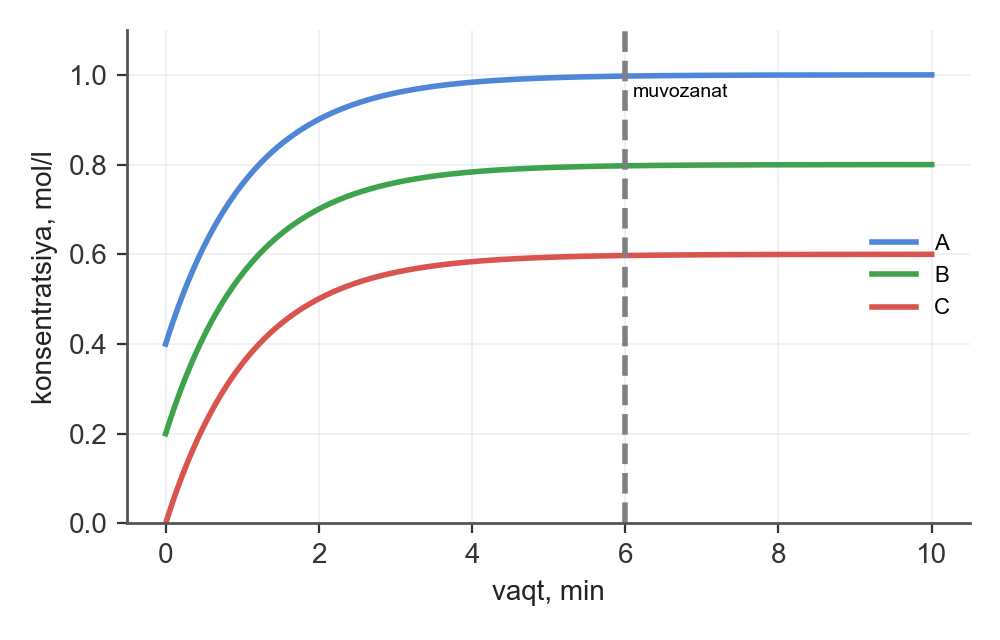
\includegraphics[width=0.86\linewidth]{rasmlar/gen/conc_v09_0.png}\end{center}
Grafikdan foydalanib, muvozanat \textbf{konstantasini (K) aniqlang.}

\noindent A)~\textsl{7,5} \hfill B)~\textsl{15} \hfill C)~\textsl{3,75} \hfill D)~\textsl{1}\par
\qsep
\noindent\qn{8.} CuSO\textsubscript{4} eritmasi inert elektrodlar yordamida 10 A tok kuchi bilan 3860 s elektroliz qilindi. Elektrolizyorning hajmi 5 l. Katodda ajralgan Cu massasi (g) \textbf{ni toping.}

\noindent A)~\textsl{25,6} \hfill B)~\textsl{6,4} \hfill C)~\textsl{5,12} \hfill D)~\textsl{12,8}\par
\qsep
\noindent\qn{9.} 240 g 10\% li KOH eritmasi inert elektrodlar bilan elektroliz qilinib, ishqorning massa ulushi 16\% ga yetdi. Elektrolizyorning hajmi 3 l. Elektrolizda ajralgan gazlarning umumiy \textbf{hajmini (l, n.sh.) hisoblang.}

\noindent A)~\textsl{112} \hfill B)~\textsl{168} \hfill C)~\textsl{336} \hfill D)~\textsl{84}\par
\qsep
\noindent\qn{10.} Jadvalda KNO\textsubscript{3} ning ikki eritmasi haqida ma'lumot berilgan:
\begin{center}
\renewcommand{\arraystretch}{1.15}
\fitbox{\begin{tabular}{|c|c|c|}\hline
\textbf{Eritma} & \textbf{Massasi, g} & \textbf{Massa ulushi, \%} \\ \hline
1 & 250 & 5 \\ \hline
2 & 150 & 25 \\ \hline
\end{tabular}}
\end{center}
Eritmalar aralashtirilib, ustiga 100 g suv qo`shildi. Hosil bo`lgan eritmaning massa \textbf{ulushini (\%) aniqlang.}

\noindent A)~\textsl{15} \hfill B)~\textsl{10} \hfill C)~\textsl{30} \hfill D)~\textsl{17,5}\par
\qsep
\noindent\qn{11.} H\textsubscript{2}O\textsubscript{2} moddaning parchalanish reaksiyasida konsentratsiyaning vaqt bo`yicha o`zgarishi jadvalda berilgan:
\begin{center}
\renewcommand{\arraystretch}{1.15}
\fitbox{\begin{tabular}{|c|c|}\hline
\textbf{t, min} & \textbf{c, mol/l} \\ \hline
0 & 2,4 \\ \hline
2 & 2,16 \\ \hline
4 & 1,92 \\ \hline
6 & 1,68 \\ \hline
\end{tabular}}
\end{center}
0-minutdan 2-minutgacha o`rtacha tezlikni mol/(l$\cdot$min) \textbf{hisoblang.}

\noindent A)~\textsl{0,12} \hfill B)~\textsl{0,24} \hfill C)~\textsl{0,06} \hfill D)~\textsl{1,2}\par
\qsep
\noindent\qn{12.} CO + H\textsubscript{2}O $\rightleftarrows$ CO\textsubscript{2} + H\textsubscript{2} reaksiyasi 1 l hajmli idishda o`tkazildi. Ma'lumotlar jadvalda berilgan:
\begin{center}
\renewcommand{\arraystretch}{1.15}
\fitbox{\begin{tabular}{|c|c|c|c|}\hline
\textbf{Modda} & \textbf{CO} & \textbf{H\textsubscript{2}O} & \textbf{CO\textsubscript{2}} \\ \hline
Boshlang`ich, mol & 6 & 2 & 0 \\ \hline
Muvozanatda, mol & --- & --- & 1,5 \\ \hline
\end{tabular}}
\end{center}
CO ning necha foizi reaksiyaga \textbf{kirishganini aniqlang.}

\noindent A)~\textsl{12,5} \hfill B)~\textsl{37,5} \hfill C)~\textsl{25} \hfill D)~\textsl{75}\par
\qsep
\noindent\qn{13.} CO + H\textsubscript{2}O $\rightleftarrows$ CO\textsubscript{2} + H\textsubscript{2} sistemasida boshlang`ich moddalarning har biridan 2 mol dan 1 l hajmli idishga solindi. Muvozanat qaror topganda reagentlarning har birining 3/5 qismi sarflangan bo`ldi. Muvozanat \textbf{konstantasini hisoblang.}

\noindent A)~\textsl{4,5} \hfill B)~\textsl{2,25} \hfill C)~\textsl{1,12} \hfill D)~\textsl{3,25}\par
\qsep
\noindent\qn{14.} Qaysi juftliklar o`zaro reaksiyaga kirishmaydi? 1) CuSO\textsubscript{4} va NaOH; 2) Na\textsubscript{2}CO\textsubscript{3} va HCl; 3) ZnO va HCl; 4) Fe va HNO\textsubscript{3}(sovuq kons.)

\noindent A)~\textsl{1, 4} \hfill B)~\textsl{4} \hfill C)~\textsl{2, 3} \hfill D)~\textsl{2, 4}\par
\qsep
\noindent\qn{15.} AgNO\textsubscript{3} qizdirilganda qanday moddalar hosil bo`ladi?

\noindent\begin{tabular}{@{}p{0.47\linewidth}@{}p{0.47\linewidth}@{}}
A)~\textsl{Ag, NO\textsubscript{2} va O\textsubscript{2}} & B)~\textsl{ZnO, NO\textsubscript{2} va O\textsubscript{2}} \\
C)~\textsl{KNO\textsubscript{2} va O\textsubscript{2}} & D)~\textsl{N\textsubscript{2}O va H\textsubscript{2}O} \\
\end{tabular}\par
\qsep
\noindent\qn{16.} 170 g ammiak katalitik oksidlanib NO ga (unum 80\%), so`ng NO\textsubscript{2} va HNO\textsubscript{3} gacha (umumiy unum 75\%) aylantirildi. Barcha reaksiyalar 1 atm bosimda olib borildi. Hosil bo`lgan nitrat kislota \textbf{massasini (g) hisoblang.}

\noindent A)~\textsl{630} \hfill B)~\textsl{756} \hfill C)~\textsl{504} \hfill D)~\textsl{378}\par
\qsep
\noindent\qn{17.} PbO va CuO aralashmasi tarkibida PbO ning massasi CuO ning massasidan 26,9 g ga ko`p. Shu aralashma vodorod bilan to`liq qaytarilganda 14,4 g suv hosil bo`ldi. Aralashmaning zichligi 2,8 g/sm\textsuperscript{3} ga teng. Aralashmadagi PbO ning \textbf{massasini (g) toping.}

\noindent A)~\textsl{40} \hfill B)~\textsl{133,8} \hfill C)~\textsl{66,9} \hfill D)~\textsl{53,45}\par
\qsep
\noindent\qn{18.} 1 l suvda 0,03 mol Ca(HCO\textsubscript{3})\textsubscript{2}, 0,01 mol CaSO\textsubscript{4} va 0,02 mol MgCl\textsubscript{2} erigan. Suv qaynatilgandan keyin qolgan qattiqlikni yo`qotish uchun necha gramm soda (Na\textsubscript{2}CO\textsubscript{3}) kerak?

\noindent A)~\textsl{3,18} \hfill B)~\textsl{6,36} \hfill C)~\textsl{1,06} \hfill D)~\textsl{2,12}\par
\qsep
\noindent\qn{19.} Fe\textsubscript{2}(SO\textsubscript{4})\textsubscript{3} va MgSO\textsubscript{4} aralashmasi tarkibida Fe\textsubscript{2}(SO\textsubscript{4})\textsubscript{3} ning mol miqdori aralashmadagi umumiy mol miqdorining 4/5 qismini tashkil etadi. Shu aralashma suvda eritilib, mo`l BaCl\textsubscript{2} qo`shilganda 302,9 g cho`kma tushdi. Aralashmadagi Fe\textsubscript{2}(SO\textsubscript{4})\textsubscript{3} ning mol \textbf{ulushini (\%) hisoblang.}

\noindent A)~\textsl{80} \hfill B)~\textsl{20} \hfill C)~\textsl{93,02} \hfill D)~\textsl{50}\par
\qsep
\noindent\qn{20.} Spirt va fenollar haqida qaysi fikrlar to`g`ri? 1) Uchlamchi spirtlar oson oksidlanadi; 2) Etanol natriy bilan reaksiyaga kirishadi; 3) Etilenglikol zaharsiz; 4) Fenol Cu(OH)\textsubscript{2} ni eritib ko`k kompleks hosil qiladi

\noindent A)~\textsl{3} \hfill B)~\textsl{2} \hfill C)~\textsl{2, 4} \hfill D)~\textsl{1, 4}\par
\qsep
\noindent\qn{21.} Karbon kislotalar haqida qaysi fikrlar to`g`ri? 1) Stearin kislota to`yinmagan kislota; 2) Sirka angidrid ikki molekula sirka kislotadan suv chiqib hosil bo`ladi; 3) Sirka kislota karbonatlar bilan CO\textsubscript{2} ajratadi; 4) Qattiq suvda sovun yaxshi ko`piklanadi

\noindent A)~\textsl{3, 4} \hfill B)~\textsl{2} \hfill C)~\textsl{2, 3} \hfill D)~\textsl{2, 3, 4}\par
\qsep
\noindent\qn{22.} Quyidagi birikmalardan qaysi biri amin sinfiga kiradi?

\noindent\begin{tabular}{@{}p{0.47\linewidth}@{}p{0.47\linewidth}@{}}
A)~\textsl{CH\textsubscript{3}OCH\textsubscript{3}} & B)~\textsl{CH\textsubscript{3}COOC\textsubscript{2}H\textsubscript{5}} \\
C)~\textsl{C\textsubscript{2}H\textsubscript{5}NH\textsubscript{2}} & D)~\textsl{CH\textsubscript{3}COOH} \\
\end{tabular}\par
\qsep
\noindent\qn{23.} Etilen va vodorod aralashmasining (mol nisbati 2 : 3) vodorodga nisbatan zichligi 6,2. Aralashma Ni katalizatori ustida to`liq gidrogenlandi. Gaz hajmi necha foizga kamayadi?

\noindent A)~\textsl{80} \hfill B)~\textsl{60} \hfill C)~\textsl{40} \hfill D)~\textsl{66,7}\par
\qsep
\noindent\qn{24.} Rasmda siklik uglevodorodning tuzilish formulasi berilgan.
\begin{center}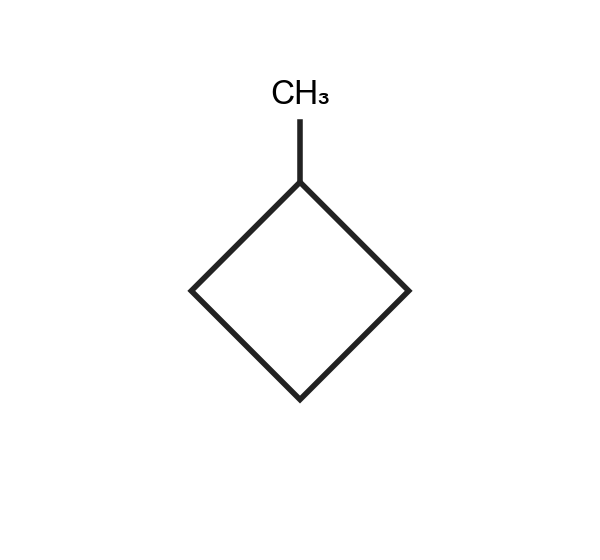
\includegraphics[width=0.86\linewidth]{rasmlar/gen/rn_800378.png}\end{center}
Birikmaning molekulyar \textbf{formulasini aniqlang.}

\noindent A)~\textsl{C\textsubscript{5}H\textsubscript{12}} \hfill B)~\textsl{C\textsubscript{6}H\textsubscript{10}} \hfill C)~\textsl{C\textsubscript{5}H\textsubscript{10}} \hfill D)~\textsl{C\textsubscript{5}H\textsubscript{8}}\par
\qsep
\noindent\qn{25.} Metilformiat va metilatsetat aralashmasi (32,8 g) mo`l NaOH eritmasi bilan to`liq gidrolizlandi. Aralashmaning mol miqdori 0,5 mol. Hosil bo`lgan tuzlar \textbf{massasini (g) aniqlang.}

\noindent A)~\textsl{73,6} \hfill B)~\textsl{32,8} \hfill C)~\textsl{37,5} \hfill D)~\textsl{36,8}\par
\qsep
\noindent\qn{26.} 448 l (n.sh.) C\textsubscript{2}H\textsubscript{6} dan quyidagi sxema bo`yicha 570,24 g etilatsetat olindi: C\textsubscript{2}H\textsubscript{6} $\to$ C\textsubscript{2}H\textsubscript{4} $\to$ C\textsubscript{2}H\textsubscript{5}OH $\to$ CH\textsubscript{3}COOC\textsubscript{2}H\textsubscript{5}. Dastlabki 2 bosqichning unumi ketma-ket 60\%, 60\% ga teng. Barcha reaksiyalar 2 atm bosimda olib borildi. Oxirgi bosqichning \textbf{unumini (\%) aniqlang.}

\noindent A)~\textsl{45} \hfill B)~\textsl{10} \hfill C)~\textsl{72} \hfill D)~\textsl{90}\par
\qsep
\noindent\qn{27.} 56 l (n.sh.) CH\textsubscript{4} dan quyidagi sxema bo`yicha 145,8 g kumush olindi: CH\textsubscript{4} $\to$ C\textsubscript{2}H\textsubscript{2} $\to$ CH\textsubscript{3}CHO $\to$ Ag. Dastlabki 2 bosqichning unumi ketma-ket 90\%, 80\% ga teng. Oxirgi bosqichning \textbf{unumini (\%) aniqlang.}

\noindent A)~\textsl{38} \hfill B)~\textsl{25} \hfill C)~\textsl{60} \hfill D)~\textsl{75}\par
\qsep
\noindent\qn{28.} 128 g CaC\textsubscript{2} dan quyidagi sxema bo`yicha polivinilxlorid olindi: CaC\textsubscript{2} $\to$ C\textsubscript{2}H\textsubscript{2} $\to$ CH\textsubscript{2}=CHCl $\to$ (--CH\textsubscript{2}--CHCl--)n. Bosqichlarning unumi ketma-ket 75\%, 75\%, 80\% ni tashkil qiladi. Barcha reaksiyalar 1,5 atm bosimda olib borildi. Olingan polivinilxlorid \textbf{massasini (g) aniqlang.}

\noindent A)~\textsl{112,5} \hfill B)~\textsl{28,12} \hfill C)~\textsl{70,31} \hfill D)~\textsl{56,25}\par
\qsep
\noindent\qn{29.} C\textsubscript{6}H\textsubscript{6} dan quyidagi sxema bo`yicha 53,04 g polistirol olindi: C\textsubscript{6}H\textsubscript{6} $\to$ C\textsubscript{6}H\textsubscript{5}--C\textsubscript{2}H\textsubscript{5} $\to$ C\textsubscript{6}H\textsubscript{5}--CH=CH\textsubscript{2} $\to$ (--CH\textsubscript{2}--CH(C\textsubscript{6}H\textsubscript{5})--)n. Bosqichlarning unumi ketma-ket 85\%, 40\%, 75\% ni tashkil qiladi. Sarflangan C\textsubscript{6}H\textsubscript{6} massasi (g) \textbf{ni aniqlang.}

\noindent A)~\textsl{312} \hfill B)~\textsl{78} \hfill C)~\textsl{156} \hfill D)~\textsl{132,6}\par
\qsep
\noindent\qn{30.} Probirkalardagi organik moddalar: fenol, etanol, etanal ni alohida probirkalarda ajratish uchun qaysi reagent(lar) yetarli? 1) [Ag(NH\textsubscript{3})\textsubscript{2}]OH va FeCl\textsubscript{3}; 2) Cu(OH)\textsubscript{2} (sovuqda) va Na metali; 3) Cu(OH)\textsubscript{2} (sovuqda) va FeCl\textsubscript{3}; 4) [Ag(NH\textsubscript{3})\textsubscript{2}]OH

\noindent A)~\textsl{2, 4} \hfill B)~\textsl{1} \hfill C)~\textsl{3} \hfill D)~\textsl{2}\par
\qsep
\noindent\qn{31.} Kimyo laboratoriyasida ishlash qoidalari haqida qaysi fikrlar to`g`ri? 1) Suvni konsentrlangan kislotaga tez quyish mumkin; 2) Zaharli gaz ajraladigan tajriba mo`rili shkafda o`tkaziladi; 3) Ortiqcha reaktiv idishga qaytariladi; 4) Ishqor teriga tushsa, qo`l suv bilan yuviladi

\noindent A)~\textsl{2, 4} \hfill B)~\textsl{1} \hfill C)~\textsl{1, 3} \hfill D)~\textsl{2, 3}\par
\qsep
\noindent\qn{32.} Rasmda tasvirlangan usul bilan qaysi aralashmani ajratish mumkin?
\begin{center}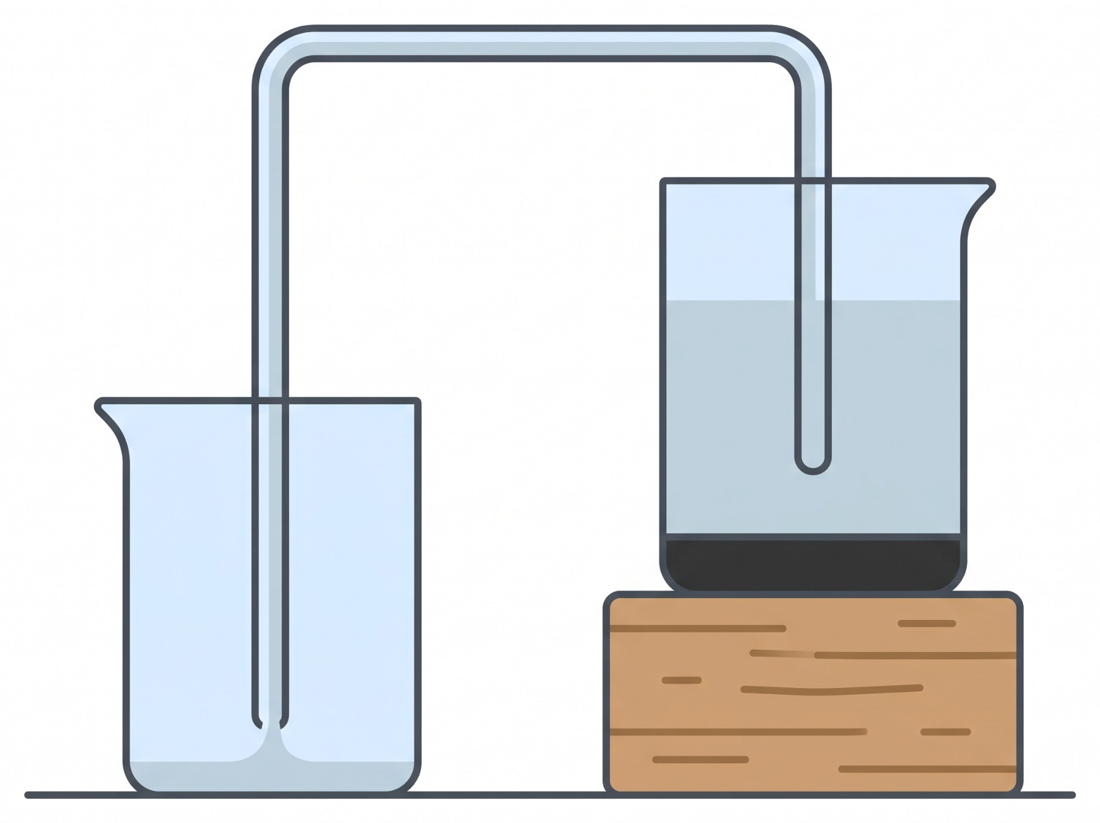
\includegraphics[width=0.86\linewidth]{rasmlar/darslik/d_tindirish.png}\end{center}
\noindent A)~\textsl{suv va etanol}\par
\noindent B)~\textsl{osh tuzi eritmasi}\par
\noindent C)~\textsl{suv va kerosin}\par
\noindent D)~\textsl{loyqa suv (suv va qum zarrachalari)   ---}\par
\qsep
\end{multicols}
\medskip
\noindent\setlength{\fboxsep}{0pt}\fbox{\begin{tabular}{p{0.74\linewidth}|p{0.2\linewidth}}
\parbox[t]{0.72\linewidth}{\vspace{3pt}\textbf{Topshiriqlar (33--35) va javob variant (A--F)larini o`zaro to`g`ri moslashtiring.} Qo`rg`oshin(II) nitratning 0,01 mol/l li eritmasidan 1000 ml olinib, inert elektrodlar yordamida 5 A tok kuchi bilan 193 s elektroliz qilindi (eritma hajmi o`zgarmadi deb hisoblang). Elektrolizdan keyin eritmaga mo`l KI eritmasi qo`shildi.
\vspace{3pt}} & \parbox[t]{0.19\linewidth}{\vspace{3pt}A~\textsl{1,6}\\[3pt]
B~\textsl{1}\\[3pt]
C~\textsl{2}\\[3pt]
D~\textsl{3,69}\\[3pt]
E~\textsl{1,03}\\[3pt]
F~\textsl{4,61}}\\ \hline
\parbox[t]{0.72\linewidth}{\vspace{2pt}\textbf{33. Katodda ajralgan qo`rg`oshin massasini (g) toping.}\vspace{2pt}} & \\ \hline
\parbox[t]{0.72\linewidth}{\vspace{2pt}\textbf{34. Elektroliz tugagach eritmaning pH ini hisoblang.}\vspace{2pt}} & \\ \hline
\parbox[t]{0.72\linewidth}{\vspace{2pt}\textbf{35. KI qo`shilganda hosil bo`lgan cho`kma massasini (g) aniqlang.}\vspace{2pt}} & 
\end{tabular}}
\par\bigskip
\noindent\qn{36.} C + HNO\textsubscript{3} $\to$ CO\textsubscript{2} + NO\textsubscript{2} + H\textsubscript{2}O reaksiya tenglamasini tenglang. Tajriba hajmi 250 ml bo`lgan kolbada o`tkazildi. Reagentlar (chap qism) koeffitsiyentlari \textbf{yig`indisini toping.}
\javob\qsep
\noindent\qn{37.} 240 g 8\% li tuz eritmasidan suv bug`latilganda tuzning massa ulushi 4/3 marta ortdi. Tajriba laboratoriyada, shisha idishda o`tkazildi. Bug`latilgan suv \textbf{massasini (g) toping.}
\javob\qsep
\noindent\qn{38.} CaCO\textsubscript{3} va MgCO\textsubscript{3} dan iborat 38,4 g aralashma doimiy massagacha qizdirilganda qoldiq massasi 20,8 g bo`ldi. Aralashmaning zichligi 2,3 g/sm\textsuperscript{3} ga teng. Aralashmadagi CaCO\textsubscript{3} ning \textbf{massasini (g) toping.}
\javob\qsep
\noindent\qn{39.} Noma'lum alkenning 22,4 g miqdori mo`l brom suvi bilan to`liq reaksiyaga kirishganda 64 g brom sarflandi. Xuddi shu alkenning 1/2 qismi gidratlanib spirtga aylantirildi, hosil bo`lgan spirt natriy bilan ta'sirlashtirildi. Reagent (brom suvi) eritmasining massa ulushi 50\% va zichligi 1,4 g/ml; u mo`l miqdorda olingan. Ajralgan vodorod \textbf{hajmini (l, n.sh.) toping.}
\javob\qsep
\noindent\qn{40.} Vodorodga nisbatan zichligi 15 bo`lgan alkanning 60 g miqdorining 1/2 qismi yorug`likda xlor bilan monoxlorlandi, hosil bo`lgan xloralkan mo`l KOH ning suvli eritmasi bilan gidrolizlandi. Reagent (KOH) eritmasining massa ulushi 10\% va zichligi 1,12 g/ml; u mo`l miqdorda olingan. Hosil bo`lgan spirtning \textbf{massasini (g) toping.}
\javob\qsep
\par\bigskip\begin{center}\textbf{\fontsize{13}{15}\selectfont YOZMA ISH}\end{center}
\noindent\qn{41.} \textbf{Topshiriqni bajarish jarayonida barcha reaksiya tenglamalarini yozing. Miqdoriy va arifmetik hisoblashlarni (unga asos bo`lgan usul yoki formulani ko`rsatgan holda) uzviy ketma-ketlikda bajaring.}\par\smallskip
500 g suvda CuSO\textsubscript{4} va NaCl dan iborat 43,7 g aralashma eritildi (tuzlarning mol nisbati 1 : 1). Aralashmaning zichligi 3,1 g/sm\textsuperscript{3} ga teng. Eritma inert elektrodlar yordamida 10 A tok kuchi bilan 5790 s elektroliz qilindi (jarayonda Cu\textsuperscript{2+} va Cl\textsuperscript{$-$} ionlari to`liq tugadi, suv ham elektrolizga uchradi).\par
\noindent 1)\ Katod va anodda ketma-ket boradigan jarayonlar tenglamalarini yozing; tuzlarning dastlabki miqdorlarini (mol) aniqlang.\par
\noindent 2)\ Katodda ajralgan mis massasini (g) va vodorod hajmini (l, n.sh.) hisoblang.\par
\noindent 3)\ Anodda ajralgan xlor va kislorod hajmlarini (l, n.sh.) toping.\par
\noindent 4)\ Elektroliz tugagach eritmaning muhitini (kislotali, neytral yoki ishqoriy) asoslang va undagi ortiqcha moddaning miqdorini (mol) aniqlang.\par
\noindent 5)\ Elektrolizdan keyin eritma massasini (g) va undagi Na\textsubscript{2}SO\textsubscript{4} ning massa ulushini (\%) hisoblang.\par
\diqqat{Mazkur topshiriq kengaytirilgan javobni talab etib, uning yechilish usuli va shu usul asosidagi barcha hisoblash amallari javoblar varaqasida aks etishi lozim.}\qsep
\noindent\qn{42.} Organik moddalarning xossalarini bilgan holda reaksiya tenglamalarini tugallang va tenglashtiring. 3- va 5-reaksiyalarda hosil bo`lgan asosiy organik mahsulotlarni sistematik nomenklatura bo`yicha nomlang. Hosil bo`lgan organik moddalarning tuzilish formulalarini yozing.\par
\noindent 1)\ CH\textsubscript{3}--CHO + H\textsubscript{2} (Ni, t) $\to$\par
\noindent 2)\ C\textsubscript{6}H\textsubscript{5}--NH\textsubscript{2} + Br\textsubscript{2} (suvli eritma) $\to$\par
\noindent 3)\ 2CH\textsubscript{3}--CH\textsubscript{2}--OH (H\textsubscript{2}SO\textsubscript{4} kons., 140 \textdegree{}C) $\to$\par
\noindent 4)\ C\textsubscript{6}H\textsubscript{5}--CH\textsubscript{3} + Cl\textsubscript{2} (yorug`lik) $\to$\par
\noindent 5)\ CH\textsubscript{3}--NH\textsubscript{2} + HCl $\to$\par
\noindent 6)\ C\textsubscript{6}H\textsubscript{5}--NO\textsubscript{2} + H\textsubscript{2} (Ni, t) $\to$\par
\noindent 7)\ HCOOCH\textsubscript{3} + NaOH (t) $\to$\par
\diqqat{Mazkur topshiriq kengaytirilgan javobni talab etib, uning yechilish usuli va shu usul asosidagi barcha hisoblash amallari javoblar varaqasida aks etishi lozim.}\qsep
\noindent\qn{43.} \textbf{Topshiriqni bajarish jarayonida barcha reaksiya tenglamalarini yozing. Miqdoriy va arifmetik hisoblashlarni (unga asos bo`lgan usul yoki formulani ko`rsatgan holda) uzviy ketma-ketlikda bajaring.}\par\smallskip
Tarkibida AgNO\textsubscript{3} va Cu(NO\textsubscript{3})\textsubscript{2} bo`lgan 400 g eritmaga temir plastinka tushirildi (Ag\textsuperscript{+} va Cu\textsuperscript{2+} ning hammasi o`rnini bosdi). Plastinkada ajralgan metallar massasi 17,2 g, plastinka massasi esa 8,8 g ga ortdi. Plastinka olingach, eritmaga mo`l NaOH eritmasi qo`shildi, hosil bo`lgan cho`kma havoda to`liq oksidlanib, so`ng doimiy massagacha kuydirildi. Reagent (NaOH) eritmasining massa ulushi 50\% va zichligi 1,4 g/ml; u mo`l miqdorda olingan. Kuydirishdan hosil bo`lgan oksid alyuminiy bilan qizdirilganda (alyuminotermiya) metall hosil bo`ldi; bu metall mo`l xlorid kislotada eritilib, ajralgan gaz qizdirilgan mis(II) oksid ustidan o`tkazildi.\par
\noindent 1)\ Barcha reaksiyalarning tenglamalarini yozing va tenglashtiring. Eritmadagi AgNO\textsubscript{3} va Cu(NO\textsubscript{3})\textsubscript{2} ning miqdorlarini (mol) toping.\par
\noindent 2)\ Eritmaga o`tgan temirning massasini (g) hisoblang.\par
\noindent 3)\ Plastinka olingandan keyin eritmadagi Fe(NO\textsubscript{3})\textsubscript{2} ning massa ulushini (\%) aniqlang. Alyuminotermiyada sarflangan alyuminiy massasini (g) hisoblang.\par
\noindent 4)\ Cho`kmani oksidlashga sarflangan kislorodning hajmini (l, n.sh.) hisoblang. Metallning xlorid kislota bilan reaksiyasida ajralgan gaz hajmini (l, n.sh.) toping.\par
\noindent 5)\ Kuydirishdan hosil bo`lgan qattiq moddaning massasini (g) toping. Gaz mis(II) oksid bilan reaksiyaga kirishganda hosil bo`lgan mis massasini (g) aniqlang.\par
\diqqat{Mazkur topshiriq kengaytirilgan javobni talab etib, uning yechilish usuli va shu usul asosidagi barcha hisoblash amallari javoblar varaqasida aks etishi lozim.}\qsep
\newpage
\noindent\textbf{\fontsize{13}{15}\selectfont 9-variant}\hfill \textbf{Javoblar kaliti}\par\smallskip\hrule\smallskip
\textit{Faqat o`qituvchi uchun.}\par\medskip
\noindent\textbf{1--32-savollar}\par\smallskip
\noindent\begin{tabular}{|c|c|c|c|c|c|c|c|c|c|c|c|c|c|c|c|}\hline
\textbf{1} & \textbf{2} & \textbf{3} & \textbf{4} & \textbf{5} & \textbf{6} & \textbf{7} & \textbf{8} & \textbf{9} & \textbf{10} & \textbf{11} & \textbf{12} & \textbf{13} & \textbf{14} & \textbf{15} & \textbf{16}\\\hline
\textsl{C} & \textsl{A} & \textsl{B} & \textsl{B} & \textsl{D} & \textsl{A} & \textsl{A} & \textsl{D} & \textsl{B} & \textsl{B} & \textsl{A} & \textsl{C} & \textsl{B} & \textsl{B} & \textsl{A} & \textsl{D}\\\hline
\textbf{17} & \textbf{18} & \textbf{19} & \textbf{20} & \textbf{21} & \textbf{22} & \textbf{23} & \textbf{24} & \textbf{25} & \textbf{26} & \textbf{27} & \textbf{28} & \textbf{29} & \textbf{30} & \textbf{31} & \textbf{32}\\\hline
\textsl{C} & \textsl{A} & \textsl{A} & \textsl{B} & \textsl{C} & \textsl{C} & \textsl{C} & \textsl{C} & \textsl{D} & \textsl{D} & \textsl{D} & \textsl{D} & \textsl{C} & \textsl{B} & \textsl{A} & \textsl{D}\\\hline
\end{tabular}\par\medskip
\noindent\textbf{33--35-savollar}\par\smallskip
\noindent\begin{tabular}{|c|c|c|}\hline \textbf{No} & \textbf{Javob} & \textbf{Qiymat}\\\hline
33 & \textsl{E} & 1,03\\\hline
34 & \textsl{C} & 2\\\hline
35 & \textsl{F} & 4,61\\\hline
\end{tabular}\par\medskip
\noindent\textbf{36--40-savollar}\par\smallskip
\noindent\begin{tabular}{|c|c|}\hline \textbf{No} & \textbf{To`g`ri javob}\\\hline
36 & 5\\\hline
37 & 60\\\hline
38 & 30\\\hline
39 & 2,24\\\hline
40 & 46\\\hline
\end{tabular}\par\medskip
\noindent\textbf{41--43-topshiriqlar: javoblar}\par\smallskip
\noindent\textbf{41-topshiriq.}\par
\noindent 1) 0,2 mol; 0,2 mol\par
\noindent 2) 12,8 g; 0,1 mol = 2,24 l\par
\noindent 3) 2,24 l; 2,24 l\par
\noindent 4) kislotali; H\textsubscript{2}SO\textsubscript{4} 0,1 mol\par
\noindent 5) 520,4 g; 2,73\%\par
\noindent\textbf{42-topshiriq.}\par
\noindent 1) CH\textsubscript{3}--CHO + H\textsubscript{2} $\to$ CH\textsubscript{3}--CH\textsubscript{2}--OH\par
\noindent 2) C\textsubscript{6}H\textsubscript{5}--NH\textsubscript{2} + 3Br\textsubscript{2} $\to$ C\textsubscript{6}H\textsubscript{2}Br\textsubscript{3}--NH\textsubscript{2}$\downarrow$ + 3HBr\par
\noindent 3) 2CH\textsubscript{3}--CH\textsubscript{2}--OH $\to$ CH\textsubscript{3}--CH\textsubscript{2}--O--CH\textsubscript{2}--CH\textsubscript{3} + H\textsubscript{2}O --- nomi: \textbf{dietil efir (etoksietan)}\par
\noindent 4) C\textsubscript{6}H\textsubscript{5}--CH\textsubscript{3} + Cl\textsubscript{2} $\to$ C\textsubscript{6}H\textsubscript{5}--CH\textsubscript{2}Cl + HCl\par
\noindent 5) CH\textsubscript{3}--NH\textsubscript{2} + HCl $\to$ [CH\textsubscript{3}--NH\textsubscript{3}]Cl --- nomi: \textbf{metilammoniy xlorid}\par
\noindent 6) C\textsubscript{6}H\textsubscript{5}--NO\textsubscript{2} + 3H\textsubscript{2} $\to$ C\textsubscript{6}H\textsubscript{5}--NH\textsubscript{2} + 2H\textsubscript{2}O\par
\noindent 7) HCOOCH\textsubscript{3} + NaOH $\to$ HCOONa + CH\textsubscript{3}OH\par
\noindent\textbf{43-topshiriq.}\par
\noindent 1) 0,1 mol; 0,1 mol\par
\noindent 2) 8,4 g\par
\noindent 3) 6,9\%; 4,05 g\par
\noindent 4) 0,84 l; 3,36 l\par
\noindent 5) 12 g; 9,6 g\par
\par\bigskip\noindent\textbf{Mavzular taqsimoti}\par\smallskip
{\small\noindent\begin{longtable}{|c|p{7.2cm}|p{5.4cm}|c|}\hline \textbf{No} & \textbf{Mavzu} & \textbf{Tekshiriladigan ko`nikma} & \textbf{Ball}\\\hline
1 & Tirkashev I bob; 8-sinf (izoelektron) & Bilim va tushunish & 1\\\hline
2 & 9-sinf; 10-sinf (tuzlar gidrolizi, ion almashinish reaksiyalari) & Bilim va tushunish & 1\\\hline
3 & 9-sinf; 11-sinf (tuzlar gidrolizi; Le-Shatelye) & Bilim va tushunish & 1\\\hline
4 & 11-sinf 4-bob (normal konsentratsiya) & Hisoblash va masala yechish & 1\\\hline
5 & 8-sinf; Tirkashev \textit{V} bob (oksidlanish darajasi) & Bilim va tushunish & 1\\\hline
6 & 8-sinf (oksidlar tarkibi; massa ulushi) & Hisoblash va masala yechish & 1\\\hline
7 & Tirkashev VI bob (muvozanat, grafik) & Grafik tahlili & 1\\\hline
8 & 11-sinf 8-bob (Faradey qonunlari); Tirkashev \textit{V} bob & Hisoblash va masala yechish & 1\\\hline
9 & 11-sinf (elektroliz; suvning elektrolizi) & Hisoblash va masala yechish & 1\\\hline
10 & Tirkashev III bob (eritmalar, jadval) & Jadval tahlili & 1\\\hline
11 & Tirkashev VI bob (tezlik, jadval) & Jadval tahlili & 1\\\hline
12 & Tirkashev VI bob (muvozanat, jadval) & Jadval tahlili & 1\\\hline
13 & 9-11-sinf (kimyoviy muvozanat) & Hisoblash va masala yechish & 1\\\hline
14 & 9-sinf; Tashev (anorganik birikmalar xossalari) & Bilim va tushunish & 1\\\hline
15 & Tashev (nitratlar) & Bilim va tushunish & 1\\\hline
16 & 9-sinf (azotning birikmalari; ammiak va HNO\textsubscript{3} olinishi) & Hisoblash va masala yechish & 1\\\hline
17 & 9-sinf (metall oksidlarining vodorod bilan qaytarilishi) & Hisoblash va masala yechish & 1\\\hline
18 & 9-sinf \S{}24 (doimiy qattiqlik, soda) & Hisoblash va masala yechish & 1\\\hline
19 & 9-sinf (sulfatlar; sifat reaksiyasi) & Hisoblash va masala yechish & 1\\\hline
20 & 10-sinf (mavzuga oid paragraflar); Abdusamatov & Bilim va tushunish & 1\\\hline
21 & 10-sinf (mavzuga oid paragraflar); Abdusamatov & Bilim va tushunish & 1\\\hline
22 & 10-sinf (organik birikmalar sinflari) & Bilim va tushunish & 1\\\hline
23 & 10-sinf (alkenlarni gidrogenlash) & Hisoblash va masala yechish & 1\\\hline
24 & 10-sinf (sikloalkanlar) & Rasm bo`yicha tahlil & 1\\\hline
25 & 10-sinf (murakkab efirlarning gidrolizi) & Hisoblash va masala yechish & 1\\\hline
26 & 10-sinf (alkanlar, alkenlar, spirtlar, efirlar) & Hisoblash va masala yechish & 1\\\hline
27 & 10-sinf (metandan atsetilen, Kucherov, kumush ko`zgu) & Hisoblash va masala yechish & 1\\\hline
28 & 10-sinf (polimerlar; vinilxlorid olinishi) & Hisoblash va masala yechish & 1\\\hline
29 & 10-sinf (arenlar, polimerlar) & Hisoblash va masala yechish & 1\\\hline
30 & 10-sinf (spirt, aldegid, fenol sifat reaksiyalari) & Bilim va tushunish & 1\\\hline
31 & 7-sinf (xavfsizlik qoidalari); 10-sinf lab. & Bilim va tushunish & 1\\\hline
32 & 7-sinf (9-rasm) & Rasm bo`yicha tahlil & 1\\\hline
33--35 & Aralash masala (moslashtirish) & Ko`p bosqichli hisob & 3\\\hline
36--40 & Qisqa javobli masalalar & Hisoblash & 5\\\hline
41--43 & Yozma ish & Usul va hisob (M, A) & 75\\\hline
\end{longtable}}
\end{document}
